\section{Implementation}

\begin{frame}
	\frametitle{The Barnes-Hut Approximation}
	\begin{enumerate}
		\item Place all the particles in a tree.
		\item For each tree node, compute the center of mass.
		\item For each particle, compute a force. Start interacting with the root level, request deeper levels if
		$$\theta<\frac{s}{d}.$$
		\item Perform a time step.
		\item \emph{Update} the tree structure.
		\item Save results if needed, go to 2 or exit.
	\end{enumerate}
\end{frame}

\begin{frame}
	\frametitle{The Barnes-Hut (Quad-)Tree}
	\begin{figure}
		\centering
		\begin{tikzpicture}[scale=0.05,%
		every circle node/.style = {width=3,fill=black}]
		\input{incl/bh-grid-build.tex}
		\end{tikzpicture}
		\caption{Sample 4-level Barnes-Hut grid with 10 particles.}
		\label{fig:bh-grid}
	\end{figure}
\end{frame}

\begin{frame}
	\frametitle{The Barnes-Hut (Quad-)Tree (Cont.)}
	\begin{figure}
		\centering
		\newlength{\lvld}
		\setlength{\lvld}{7em}
		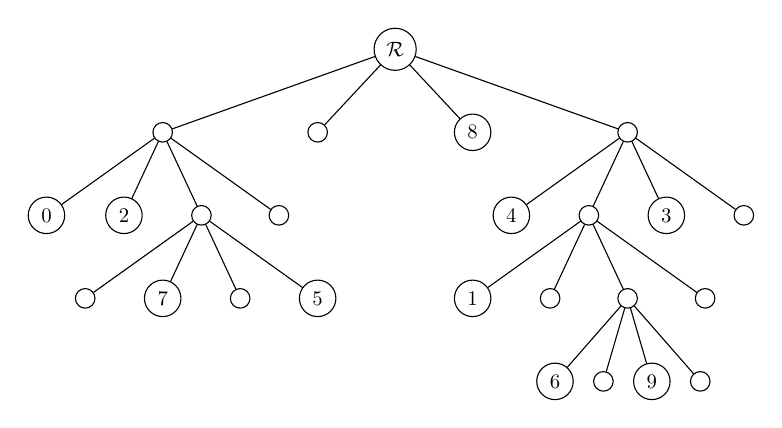
\begin{tikzpicture}[level distance=3em,
		sibling distance=3em,
		level 1/.style={sibling distance=0.80\lvld},
		level 2/.style={sibling distance=0.40\lvld},
		level 3/.style={sibling distance=0.4\lvld},
		level 4/.style={sibling distance=0.25\lvld},
		every node/.style = {shape=circle, draw, align=center, color=black,
			fill=white, scale=0.75}]
		\node {$\mathcal{R}$} %Root
child { node {} %1SW
	child { node{0} } %2SW
	child { node{2} } %2NW
	child { node{} %2SE
		child { node{} } %3SW
		child { node{7} } %3NW
		child { node{} } %3SE
		child { node{5} } } %3NE
	child { node{} } } %2NE
child { node{} }%1NW
child { node{8} }%1SE
child { node{} %1NE
	child { node{4} } %2SW
	child { node{} %2NW
		child { node {1} } %3SW
		child { node {} } %3NW
		child { node {} %3SE
			child { node{6} } %4SW
			child { node{} } %4NW
			child { node{9} } %4SE
			child { node{} } %4SW
		}
		child { node {} } }%3NE
	child { node{3} } %2SE
	child{ node{} } }; %2NE
		\end{tikzpicture}
		\caption{Tree structure associated to the configuration depicted in \cref{fig:bh-grid}.}
	\end{figure}
\end{frame}

\begin{frame}
	\frametitle{Data Structures}
	To compute forces, all we need is information about the centers of mass. In the code,
	\begin{itemize}
		\item A \lstinline{Particle} describes a center of mass (mass, position, velocity, acceleration).
		\item A \lstinline{Node} is a \lstinline{Particle} wrapper. It gives a center of mass information about its surrounding (geometrical boundaries, parent, children).
		\item A \lstinline{QuadTree} manages \lstinline{Node} objects. It provides methods to browse the tree.
		\item A \lstinline{Simulation} manages the run, times it (with \lstinline|Timer|) including IO (via \lstinline{IOManager}).
	\end{itemize}
\end{frame}

\begin{frame}
	\frametitle{Data Structures (Cont.)}
	\begin{figure}
		\centering
		\includegraphics[width=0.5\textwidth]{inclfigs/class_simulation.png}
		\caption{Collaboration graph of the \lstinline|Simulation| class.}
	\end{figure}
\end{frame}

\begin{frame}
	\frametitle{Data Structures (Cont.)}
	Computation of the force should be the main task. Avoid memory latency issues if possible?
	\begin{itemize}
		\item<1-> SoA vs. \only<1>{AoS}\only<2->{\alert{AoS}}: SoA feasible on one CPU. However,
		\begin{itemize}
			\item Parallelized problem managing only some particles?
			\item Particles being passed after time evolution?
			\item Runaway particles?
		\end{itemize}
		\item<2-> \only<2>{Pointers}\only<3->{\alert{Pointers}} or array in the tree?
		\begin{itemize}
			\item Inhomogeneous particle distributions, most nodes empty.
			\item Using arrays means allocating full levels, exponentially increasing memory usage.
		\end{itemize}
	\end{itemize}

	\onslide<3->{However, the ``physical'' particles being simulated are kept local to another in a separate storage (in \lstinline|SConfig|).}
\end{frame}

\begin{frame}[t]
\frametitle{Recursion}
Up to v0.5 (FMM attempt), code was written with recursive instructions. With \only<1>{\lstinline|O0|}\only<2>{\lstinline|O3|},
\begin{columns}
	\begin{column}{0.7\textwidth}
		\only<1>{\lstinputlisting[basicstyle=\tiny]{incl/perf.o0.hist.0}}
		\only<2>{\lstinputlisting[basicstyle=\tiny]{incl/perf.o3.hist.0}}
	\end{column}
	\begin{column}{0.3\textwidth}
		\only<1>{\SI{49.92}{\second} per iter.}\only<2>{\SI{6.45}{\second} per iter.}
		
		\only<1>{3 iterations sampled:\SI{149.75}{\second}}\only<2>{3 iterations sampled:\SI{129.07}{\second}}
	\end{column}
\end{columns}
\end{frame}

\begin{frame}
	\frametitle{Recursion (Cont.)}
	The compiler ``mysteriously'' destroys the recursive calls with enough optimization.
	
	All methods in the Barnes-Hut code avoid recursive calls.
	\begin{itemize}
		\item Much deeper levels possible for unbalanced problems. Stack could become large.
		\item More switch statements, but removes class inheritance (and thus virtual calls!).
	\end{itemize}
\end{frame}
